\documentclass{beamer}

\usepackage{ucs}
\usepackage[utf8x]{inputenc}
\usepackage[T1]{fontenc}
\usepackage[english]{babel}
\usepackage{epstopdf}

%\usepackage{multirow}%	multirow
%\usepackage[retainorgcmds]{IEEEtrantools}%	IEEEeqnarray
%\usepackage{mathabx}%	convolution symbol
\usepackage{relsize}%	relative font sizes
%\usepackage{listings}
\usepackage{graphicx}
\usepackage{multicol}


%	presentation info
\title{Parallel Sorting}
\subtitle{Samplesort}

\author{Pedro Costa}

\institute[19830]{
	University of Minho\\
	Department of Informatics
}

\date{Braga, May 2012}


%	beamer options
\usetheme{CambridgeUS}


\begin{document}%	begin presentation

\maketitle%	title slide

\frame{\frametitle{Index}\tableofcontents}

\section{Samplesort}
\frame{\frametitle{Index}\tableofcontents[currentsection,currentsubsection]}

\begin{frame}
	\frametitle{PSRS}

		\begin{center}
			\huge\bfseries Why?
		\end{center}
		
	\begin{enumerate}
		\item{From \cite{Quinn2004}:
		\begin{quote}
			\textbf{Parallel sorting by regular sampling} (PSRS), developed by Li et al. \cite{Li1993}, has three advantages over hyperquicksort. It keeps list sizes more balanced among the processes, it avoids repeated communications of the keys, and it does not require that the number of processes be a power of 2.
		\end{quote}
		}
		\item{Very high ``score'' in \cite{Kale2010};}
		\item{Quicksort does not offer a challenge;}
		\item{It's awesome.}
	\end{enumerate}
\end{frame}











\subsection{Algorithm}
\frame{\frametitle{Index}\tableofcontents[currentsection,currentsubsection]}









\begin{frame}
	\frametitle{Partition}
	\begin{figure}
		\begin{center}
			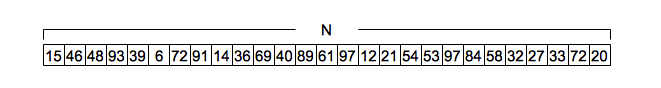
\includegraphics[width=\textwidth]{images/00start.png}
		\end{center}
	\end{figure}
	
	\begin{itemize}
		\item{A set of $n$ keys to order.}
		\pause
		\item{Divide over $p$ processes.}
	\end{itemize}
	
	\begin{figure}
		\begin{center}
			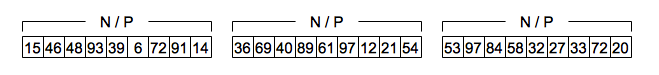
\includegraphics[width=\textwidth]{images/01partition.png}
		\end{center}
	\end{figure}
\end{frame}










\begin{frame}
	\frametitle{Local sorting}
	\begin{figure}
		\begin{center}
			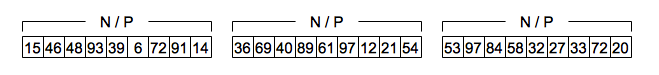
\includegraphics[width=\textwidth]{images/01partition.png}
		\end{center}
	\end{figure}
	
	\pause
	\begin{itemize}
		\item{Each process uses the \textit{quicksort} algorithm.}
	\end{itemize}
	
	\begin{figure}
		\begin{center}
			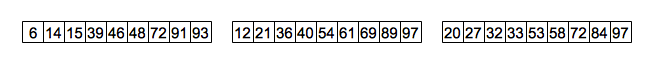
\includegraphics[width=\textwidth]{images/02localorder.png}
		\end{center}
	\end{figure}
\end{frame}










\begin{frame}
	\frametitle{Sampling}
	\begin{figure}
		\begin{center}
			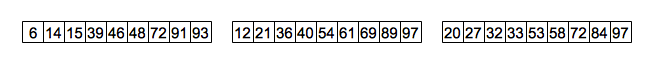
\includegraphics[width=\textwidth]{images/02localorder.png}
		\end{center}
	\end{figure}
	
	\pause
	\begin{itemize}
		\item{Each process selects $p$ samples:
		\begin{itemize}
			\item{Samplesort variants focus on the sampling rule;}
			\item{Regular Sampling = samples taken at regular intervals.}
		\end{itemize}
		}
	\end{itemize}
	
	\begin{figure}
		\begin{center}
			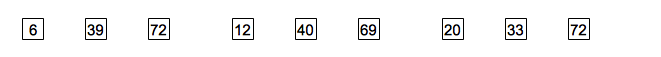
\includegraphics[width=\textwidth]{images/03sampling.png}
		\end{center}
	\end{figure}
	
	\pause
	\begin{itemize}
		\item{Each process sends its samples to the master.}
	\end{itemize}
\end{frame}










\begin{frame}
	\frametitle{Sort samples}
	\begin{figure}
		\begin{center}
			
\includegraphics[width=\textwidth]{images/03sampling2.png}
		\end{center}
	\end{figure}
	
	\pause
	\begin{itemize}
		\item{Master uses \textit{quicksort} to sort the collected samples.}
	\end{itemize}
	
	\begin{figure}
		\begin{center}
			
\includegraphics[width=\textwidth]{images/04samporder.png}
		\end{center}
	\end{figure}
\end{frame}










\begin{frame}
	\frametitle{Pivots}
	\begin{figure}
		\begin{center}
			
\includegraphics[width=\textwidth]{images/04samporder.png}
		\end{center}
	\end{figure}
	
	\pause
	\begin{itemize}
		\item{Master selects $p-1$ pivots:
		\begin{itemize}
			\item{Rule depends on the algorithm variant;}
			\item{Regular Sampling = regular intervals.}
		\end{itemize}
		}
	\end{itemize}
	
	\begin{figure}
		\begin{center}
			
\includegraphics[width=\textwidth]{images/05pivots.png}
		\end{center}
	\end{figure}
	
	\pause
	\begin{itemize}
		\item{Master broadcasts the selected pivots.}
	\end{itemize}
\end{frame}










\begin{frame}
	\frametitle{Slices}
	\begin{figure}
		\begin{center}
			
\includegraphics[width=\textwidth]{images/05pivots.png}
		\end{center}
	\end{figure}
	
	\pause
	\begin{itemize}
		\item{Each process divides its partition according to the pivots:
		\begin{itemize}
			\item{$\leq$ to the left;}
			\item{$>$ to the right;}
		\end{itemize}
		}
	\end{itemize}
	
	\begin{figure}
		\begin{center}
			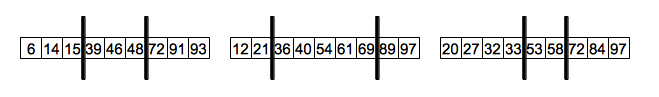
\includegraphics[width=\textwidth]{images/06slices.png}
		\end{center}
	\end{figure}
	
	\pause
	\begin{itemize}
		\item{Each process ends up with $p$ slices.}
	\end{itemize}
\end{frame}










\begin{frame}
	\frametitle{Trade}
	\begin{figure}
		\begin{center}
			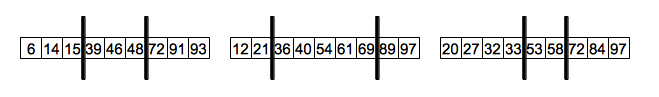
\includegraphics[width=\textwidth]{images/06slices.png}
		\end{center}
	\end{figure}
	
	\pause
	\begin{itemize}
		\item{Each process sends each $k^{\mathrm{th}}$ slice to the $k^{\mathrm{th}}$ process.}
	\end{itemize}
	
	\begin{figure}
		\begin{center}
			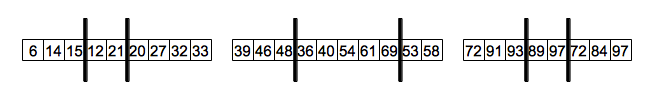
\includegraphics[width=\textwidth]{images/07trade.png}
		\end{center}
	\end{figure}
	
	\pause
	\begin{itemize}
		\item{The resulting partitions reflect the division according to the pivots.}
	\end{itemize}
\end{frame}










\begin{frame}
	\frametitle{Local sort (part 2)}
	\begin{figure}
		\begin{center}
			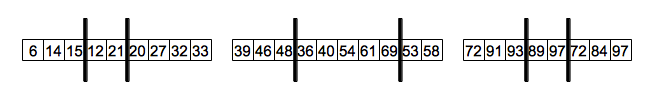
\includegraphics[width=\textwidth]{images/07trade.png}
		\end{center}
	\end{figure}
	
	\pause
	\begin{itemize}
		\item{Each process uses the \textit{quicksort} algorithm once more.}
	\end{itemize}
	
	\begin{figure}
		\begin{center}
			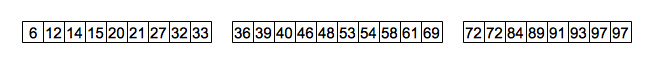
\includegraphics[width=\textwidth]{images/08localorder2.png}
		\end{center}
	\end{figure}
\end{frame}










\begin{frame}
	\frametitle{Gather}
	\begin{figure}
		\begin{center}
			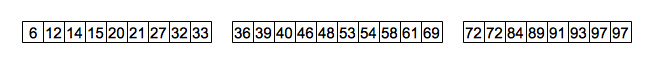
\includegraphics[width=\textwidth]{images/08localorder2.png}
		\end{center}
	\end{figure}
	
	\begin{itemize}
		\item{Each process sends its partition to the master.}
	\end{itemize}
	
	\pause
	\begin{figure}
		\begin{center}
			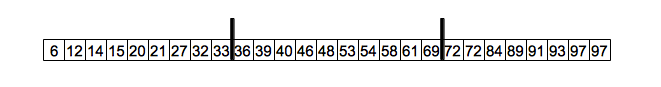
\includegraphics[width=\textwidth]{images/09final.png}
		\end{center}
	\end{figure}
	
	\begin{itemize}
		\item{The concatenation of the partitions gives the sorted set.}
	\end{itemize}
\end{frame}










\section{Implementation}
\frame{\frametitle{Index}\tableofcontents[currentsection,currentsubsection]}






\subsection{Distributed Memory}
\begin{frame}
	\frametitle{MPI}
	\begin{itemize}
		\item{Process 0 reads keys from file, calculates partition sizes and sends the partitions to each other process;}
		\pause
		\item{Local sorting with quicksort;}
		\pause
		\item{Sampling;}
		\pause
		\item{Process 0 sorts samples, collects pivots and broadcasts;}
		\pause
		\item{Each process calculates where to slice;}
		\pause
		\item{Trade: first sizes, then content;}
		\pause
		\item{Local sorting, again;}
		\pause
		\item{Every process sends its partition to process 0;}
		\pause
		\item{Process 0 outputs the result;}
	\end{itemize}
\end{frame}












\subsection{Shared Memory}
\begin{frame}
	\frametitle{OpenMP}
	\begin{itemize}
		\item{Master thread reads keys from file and calculates partitions (size and offset);}
		\pause
		\item{Local sorting with quicksort;}
		\pause
		\item{Collect samples and save in a global array;}
		\pause
		\item{Master sorts samples, collects pivots and saves in a global array;}
		\pause
		\item{Each thread calculates where to slice;}
		\pause
		\item{Trade-Sort-Gather:
		\begin{itemize}
			\item{Master reserves the memory for the sorted array;}
			\item{Each thread calculates the size of the new partition and copies from old array;}
			\item{Each thread sorts its new partition;}
		\end{itemize}
		}
		\pause
		\item{Master thread outputs the result;}
	\end{itemize}
\end{frame}









\section{Comparison}
\frame{\frametitle{Index}\tableofcontents[currentsection,currentsubsection]}






\begin{frame}
	\frametitle{Results@hex}
	\begin{figure}
		\begin{center}
			\includegraphics[width=0.95\textwidth]{images/hex-speedups.png}
		\end{center}
	\end{figure}
\end{frame}









\begin{frame}
	\frametitle{Results@511}
	\begin{figure}
		\begin{center}
			\includegraphics[width=0.95\textwidth]{images/511-speedups.png}
		\end{center}
	\end{figure}
\end{frame}








\begin{frame}
	\frametitle{Results@101}
	\begin{figure}
		\begin{center}
			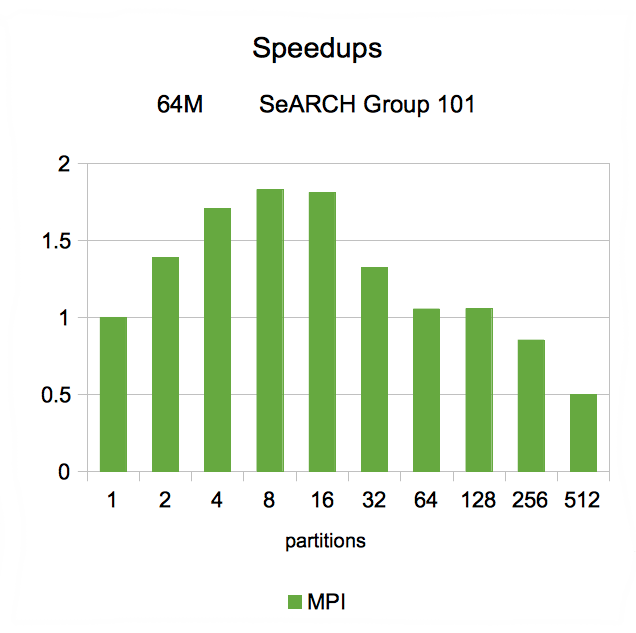
\includegraphics[width=0.6\textwidth]{images/101-speedups-mpi.png}
		\end{center}
	\end{figure}
\end{frame}







\section{Conclusion}
\begin{frame}
	\frametitle{Conclusion}
	\begin{itemize}\itemsep=20pt
		\item{The algorithm is better suited for shared memory
		\begin{itemize}
			\item{The number of keys to sort must be a lot larger for distributed memory to stand out.}
		\end{itemize}
		}
		\item{HyperThreading reduces the performance to values near MPI.}
		\item{
		\begin{description}\itemsep=10pt
			\item[OpenMP]{
			\begin{itemize}
				\item{Merge parallel zones;}
				\item{More threads vs. more partitions/thread;}
			\end{itemize}
			}
			\item[MPI]{
			\begin{itemize}
				\item{Increase $n$;}
				\item{Optimized directives;}
			\end{itemize}
			}
		\end{description}
		}
	\end{itemize}
\end{frame}






\begin{frame}
	\frametitle{Bibliography}
	\bibliographystyle{cell}
	\bibliography{slides}
\end{frame}




\section{Questions}
\begin{frame}
	\titlepage
	\begin{center}
		\Huge\bfseries
		- ? -
	\end{center}
\end{frame}

\end{document}%	end presentation
